\documentclass{article}

\usepackage[utf8]{inputenc}
\usepackage[margin=1in]{geometry}
\usepackage{amsmath, amssymb, amsthm}
% enumitem not available in this TeX installation
\usepackage{hyperref}
\usepackage{booktabs}
\usepackage{tikz}
\usetikzlibrary{arrows.meta, positioning, calc}

% --- Theorem environments ---
\newtheorem{theorem}{Theorem}[section]
\newtheorem{lemma}[theorem]{Lemma}
\newtheorem{corollary}[theorem]{Corollary}
\newtheorem{definition}[theorem]{Definition}
\newtheorem{example}{Example}[section]

\theoremstyle{remark}
\newtheorem*{remark}{Remark}

% --- Indent subsection headings and content ---
\newlength{\subsecindent}
\setlength{\subsecindent}{2em}

\makeatletter
\renewcommand\subsection{\@startsection{subsection}{2}{\subsecindent}%
  {-3.25ex\@plus -1ex \@minus -.2ex}%
  {1.5ex \@plus .2ex}%
  {\normalfont\large\bfseries}}
\makeatother

\newenvironment{sub}{%
  \begin{list}{}{%
    \setlength{\leftmargin}{4em}%
    \setlength{\rightmargin}{0pt}%
    \setlength{\topsep}{0pt}%
    \setlength{\partopsep}{0pt}%
    \setlength{\parsep}{\parskip}%
    \setlength{\itemsep}{\parskip}%
  }\item\relax
}{\end{list}}

\newenvironment{secbody}{%
  \begin{list}{}{%
    \setlength{\leftmargin}{\subsecindent}%
    \setlength{\rightmargin}{0pt}%
    \setlength{\topsep}{0pt}%
    \setlength{\partopsep}{0pt}%
    \setlength{\parsep}{\parskip}%
    \setlength{\itemsep}{\parskip}%
  }\item\relax
}{\end{list}}

% --- Custom commands ---
\newcommand{\Prob}{\mathbb{P}}
\newcommand{\given}{\mid}

\title{Bayes' Theorem: From Foundations to Applications}
\author{A Gentle Introduction}
\date{\today}

\begin{document}
\maketitle
\tableofcontents
\newpage

% ==========================================================
\section{Prerequisites: Probability Basics}
\label{sec:prereq}
% ==========================================================

\begin{secbody}
Before stating Bayes' theorem, we review the essential building blocks.
\end{secbody}

\subsection{Sample Space and Events}
\begin{sub}

\begin{definition}[Sample Space]
  A \textbf{sample space} $\Omega$ is the set of all possible outcomes of an
  experiment. An \textbf{event} $A \subseteq \Omega$ is any subset of the
  sample space.
\end{definition}

\begin{example}
  Rolling a six-sided die gives $\Omega = \{1, 2, 3, 4, 5, 6\}$.
  The event ``rolling an even number'' is $A = \{2, 4, 6\}$.
\end{example}

\end{sub}

\subsection{Axioms of Probability}
\begin{sub}

A probability measure $\Prob$ on $\Omega$ satisfies the
\emph{Kolmogorov axioms}:
\begin{enumerate}
  \item \textbf{Non-negativity:} $\Prob(A) \geq 0$ for every event $A$.
  \item \textbf{Normalization:} $\Prob(\Omega) = 1$.
  \item \textbf{Countable additivity:} If $A_1, A_2, \ldots$ are pairwise
        disjoint, then
        \[
          \Prob\!\left(\bigcup_{i=1}^{\infty} A_i\right)
          = \sum_{i=1}^{\infty} \Prob(A_i).
        \]
\end{enumerate}

From these axioms one can derive useful properties:

\begin{itemize}
  \item $\Prob(A^c) = 1 - \Prob(A)$
  \item $\Prob(\varnothing) = 0$
  \item $A \subseteq B \implies \Prob(A) \leq \Prob(B)$
  \item $\Prob(A \cup B) = \Prob(A) + \Prob(B) - \Prob(A \cap B)$
\end{itemize}

\end{sub}

\subsection{Conditional Probability}
\begin{sub}

\begin{figure}[h]
  \centering
  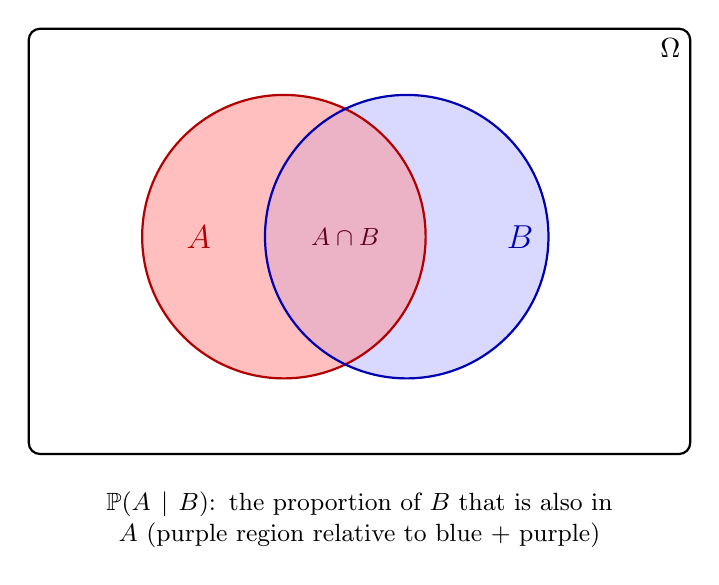
\begin{tikzpicture}[scale=1.2]
    % Sample space
    \draw[thick, rounded corners] (-3,-2) rectangle (4,2.5);
    \node[anchor=north east] at (4,2.5) {$\Omega$};

    % Event circles
    \begin{scope}[even odd rule]
      % B circle filled
      \fill[blue!15] (1,0.3) circle (1.5);
      % A cap B
      \fill[red!25] (-0.3,0.3) circle (1.5);
      \begin{scope}
        \clip (1,0.3) circle (1.5);
        \fill[purple!30] (-0.3,0.3) circle (1.5);
      \end{scope}
    \end{scope}

    \draw[thick, red!70!black]  (-0.3,0.3) circle (1.5);
    \draw[thick, blue!70!black] (1,0.3)    circle (1.5);

    % Labels
    \node[red!70!black, font=\large]  at (-1.2,0.3) {$A$};
    \node[blue!70!black, font=\large] at (2.2,0.3)  {$B$};
    \node[purple!50!black, font=\small] at (0.35,0.3) {$A \cap B$};

    % Caption below
    \node[anchor=north, font=\small, text width=7cm, align=center]
      at (0.5,-2.3) {$\Prob(A \given B)$: the proportion of $B$
      that is also in $A$ (purple region relative to blue $+$ purple)};
  \end{tikzpicture}
  \caption{Venn diagram for conditional probability}
  \label{fig:venn}
\end{figure}

\begin{definition}[Conditional Probability]
  \label{def:cond}
  For events $A$ and $B$ with $\Prob(B) > 0$, the \textbf{conditional
  probability} of $A$ given $B$ is
  \begin{equation}
    \Prob(A \given B) = \frac{\Prob(A \cap B)}{\Prob(B)}.
    \label{eq:cond}
  \end{equation}
\end{definition}

\begin{remark}
  Equation~\eqref{eq:cond} can be rearranged to obtain the
  \textbf{multiplication rule}:
  \[
    \Prob(A \cap B) = \Prob(A \given B)\,\Prob(B)
                    = \Prob(B \given A)\,\Prob(A).
  \]
\end{remark}

\end{sub}

\subsection{Law of Total Probability}
\begin{sub}

\begin{theorem}[Law of Total Probability]
  \label{thm:total}
  Let $\{B_1, B_2, \ldots, B_n\}$ be a \textbf{partition} of $\Omega$,
  i.e.\ the $B_i$ are pairwise disjoint and
  $\bigcup_{i=1}^{n} B_i = \Omega$, with $\Prob(B_i) > 0$ for all $i$.
  Then for any event $A$,
  \begin{equation}
    \Prob(A) = \sum_{i=1}^{n} \Prob(A \given B_i)\,\Prob(B_i).
    \label{eq:total}
  \end{equation}
\end{theorem}

\begin{proof}
  Since $\{B_i\}$ partitions $\Omega$,
  \[
    A = A \cap \Omega
      = A \cap \left(\bigcup_{i=1}^{n} B_i\right)
      = \bigcup_{i=1}^{n} (A \cap B_i).
  \]
  The sets $A \cap B_i$ are pairwise disjoint, so by countable additivity,
  \[
    \Prob(A)
    = \sum_{i=1}^{n} \Prob(A \cap B_i)
    = \sum_{i=1}^{n} \Prob(A \given B_i)\,\Prob(B_i). \qedhere
  \]
\end{proof}

\end{sub}

% ==========================================================
\newpage
\section{Bayes' Theorem}
\label{sec:bayes}
% ==========================================================

\subsection{Statement}
\begin{sub}

\begin{figure}[h]
  \centering
  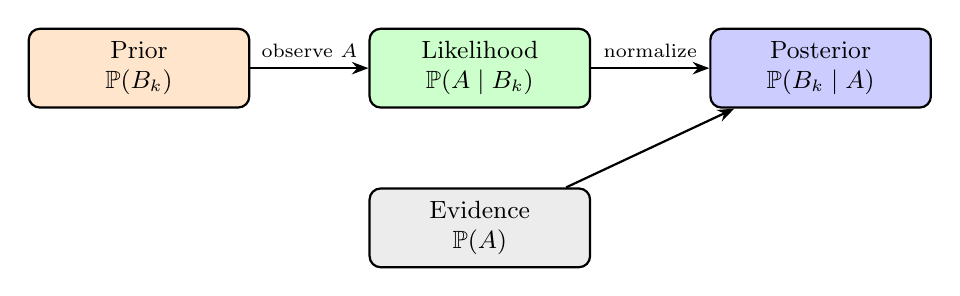
\begin{tikzpicture}[
    box/.style={draw, thick, rounded corners, minimum width=2.8cm,
                minimum height=1cm, align=center, font=\small},
    arr/.style={-{Stealth[length=6pt]}, thick},
  ]
    \node[box, fill=orange!20]  (prior)      {Prior\\$\Prob(B_k)$};
    \node[box, fill=green!20]   (like)  [right=1.5cm of prior]
      {Likelihood\\$\Prob(A \given B_k)$};
    \node[box, fill=gray!15]    (evid)  [below=1cm of like]
      {Evidence\\$\Prob(A)$};
    \node[box, fill=blue!20]    (post)  [right=1.5cm of like]
      {Posterior\\$\Prob(B_k \given A)$};

    \draw[arr] (prior) -- (like) node[midway, above, font=\scriptsize] {observe $A$};
    \draw[arr] (like)  -- (post) node[midway, above, font=\scriptsize] {normalize};
    \draw[arr] (evid)  -- (post) node[midway, right, font=\scriptsize] {};
  \end{tikzpicture}
  \caption{The Bayesian update flow: prior belief is combined with
           the likelihood of observed data and normalized by the
           evidence to produce the posterior.}
  \label{fig:flow}
\end{figure}

\begin{theorem}[Bayes' Theorem]
  \label{thm:bayes}
  Let $\{B_1, B_2, \ldots, B_n\}$ be a partition of $\Omega$ with
  $\Prob(B_i) > 0$ for all $i$, and let $A$ be an event with
  $\Prob(A) > 0$. Then for each $k = 1, \ldots, n$,
  \begin{equation}
    \boxed{\;
      \Prob(B_k \given A)
      = \frac{\Prob(A \given B_k)\,\Prob(B_k)}
             {\displaystyle\sum_{i=1}^{n} \Prob(A \given B_i)\,\Prob(B_i)}
    \;}
    \label{eq:bayes}
  \end{equation}
\end{theorem}

The terms in~\eqref{eq:bayes} have standard names:

\begin{center}
  \begin{tabular}{lll}
    \toprule
    \textbf{Term} & \textbf{Name} & \textbf{Interpretation} \\
    \midrule
    $\Prob(B_k)$          & Prior       & Belief \emph{before} observing $A$ \\
    $\Prob(A \given B_k)$ & Likelihood  & How likely $A$ is under hypothesis $B_k$ \\
    $\Prob(B_k \given A)$ & Posterior   & Updated belief \emph{after} observing $A$ \\
    $\Prob(A)$            & Evidence    & Total probability of the data \\
    \bottomrule
  \end{tabular}
\end{center}

In short:
\[
  \underbrace{\Prob(B_k \given A)}_{\text{Posterior}}
  = \frac{
      \overbrace{\Prob(A \given B_k)}^{\text{Likelihood}}
      \;\times\;
      \overbrace{\Prob(B_k)}^{\text{Prior}}
    }{
      \underbrace{\Prob(A)}_{\text{Evidence}}
    }.
\]

\end{sub}

\subsection{Proof}
\label{sec:proof}
\begin{sub}

\begin{proof}
  Starting from Definition~\ref{def:cond},
  \begin{align}
    \Prob(B_k \given A)
      &= \frac{\Prob(A \cap B_k)}{\Prob(A)}
         \label{eq:step1} \\[6pt]
      &= \frac{\Prob(A \given B_k)\,\Prob(B_k)}{\Prob(A)}
         \label{eq:step2} \\[6pt]
      &= \frac{\Prob(A \given B_k)\,\Prob(B_k)}
              {\displaystyle\sum_{i=1}^{n}
               \Prob(A \given B_i)\,\Prob(B_i)}.
         \label{eq:step3}
  \end{align}
  Step~\eqref{eq:step1} is the definition of conditional probability.
  Step~\eqref{eq:step2} applies the multiplication rule to the numerator.
  Step~\eqref{eq:step3} expands the denominator using the Law of Total
  Probability (Theorem~\ref{thm:total}).
\end{proof}

\end{sub}

% ==========================================================
\newpage
\section{Why Bayes' Theorem Matters}
\label{sec:why}
% ==========================================================

\begin{secbody}
Bayes' theorem is far more than an algebraic identity --- it is a
\emph{framework for updating beliefs in the face of new evidence}.

\begin{enumerate}
  \item \textbf{Inverse reasoning.}
    We often know $\Prob(A \given B)$ but need $\Prob(B \given A)$.
    For example, medical tests tell us
    $\Prob(\text{positive} \given \text{disease})$, but patients want
    $\Prob(\text{disease} \given \text{positive})$.

  \item \textbf{Prior $\to$ Posterior updating.}
    Bayes' theorem gives a principled mechanism for incorporating new data
    into existing knowledge.  This is the cornerstone of
    \emph{Bayesian statistics}.

  \item \textbf{Broad applicability.}
    Spam filtering, machine learning (na\"ive Bayes classifiers),
    forensic DNA analysis, clinical diagnosis, search-and-rescue
    operations, and even courtroom reasoning all rely on Bayesian
    inference.
\end{enumerate}

A common pitfall --- the \textbf{base rate fallacy} --- arises precisely
when people ignore the prior $\Prob(B_k)$. Bayes' theorem forces us to
account for it.
\end{secbody}

% ==========================================================
\newpage
\section{Worked Examples}
\label{sec:examples}
% ==========================================================

% ----------------------------------------------------------
\subsection{Medical Testing}
\label{sec:medical}
% ----------------------------------------------------------
\begin{sub}

\begin{example}[Screening for a rare disease]
  \label{ex:medical}
  A disease affects $1$ in $1{,}000$ people. A screening test has:
  \begin{itemize}
    \item \textbf{Sensitivity} (true positive rate):
          $\Prob(+ \given D) = 0.99$
    \item \textbf{Specificity} (true negative rate):
          $\Prob(- \given D^c) = 0.95$
  \end{itemize}
  \textbf{Question:} If a person tests positive, what is
  $\Prob(D \given +)$?
\end{example}

\textbf{Solution.}
The following probability tree visualizes every branch:

\begin{figure}[h]
  \centering
  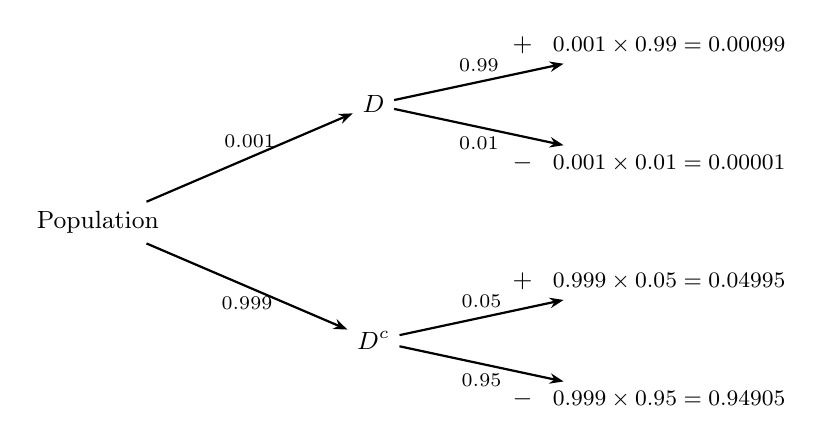
\begin{tikzpicture}[
    grow=right,
    level 1/.style={sibling distance=3cm, level distance=3.5cm},
    level 2/.style={sibling distance=1.5cm, level distance=3.5cm},
    edge from parent/.style={draw, thick, -{Stealth[length=5pt]}},
    every node/.style={font=\small},
    prob/.style={font=\scriptsize, midway},
    leaf/.style={font=\small\ttfamily},
  ]
    \node {Population}
      child {
        node {$D^c$}
        child {
          node[leaf] {$-$\; {\footnotesize $0.999 \times 0.95 = 0.94905$}}
          edge from parent node[prob, below] {$0.95$}
        }
        child {
          node[leaf] {$+$\; {\footnotesize $0.999 \times 0.05 = 0.04995$}}
          edge from parent node[prob, above] {$0.05$}
        }
        edge from parent node[prob, below] {$0.999$}
      }
      child {
        node {$D$}
        child {
          node[leaf] {$-$\; {\footnotesize $0.001 \times 0.01 = 0.00001$}}
          edge from parent node[prob, below] {$0.01$}
        }
        child {
          node[leaf] {$+$\; {\footnotesize $0.001 \times 0.99 = 0.00099$}}
          edge from parent node[prob, above] {$0.99$}
        }
        edge from parent node[prob, above] {$0.001$}
      };
  \end{tikzpicture}
  \caption{Probability tree for the medical screening example.
           The two ``$+$'' leaves give $\Prob(+) = 0.00099 + 0.04995 = 0.05094$.}
  \label{fig:tree}
\end{figure}

Define the prior and likelihood:
\begin{align*}
  \Prob(D)   &= 0.001,  &  \Prob(D^c) &= 0.999, \\
  \Prob(+ \given D)   &= 0.99,  &
  \Prob(+ \given D^c) &= 1 - 0.95 = 0.05.
\end{align*}

First, compute the total probability of a positive test using
Equation~\eqref{eq:total}:
\begin{align*}
  \Prob(+)
    &= \Prob(+ \given D)\,\Prob(D)
     + \Prob(+ \given D^c)\,\Prob(D^c) \\
    &= (0.99)(0.001) + (0.05)(0.999) \\
    &= 0.00099 + 0.04995 \\
    &= 0.05094.
\end{align*}

Now apply Bayes' theorem:
\[
  \Prob(D \given +)
  = \frac{\Prob(+ \given D)\,\Prob(D)}{\Prob(+)}
  = \frac{0.00099}{0.05094}
  \approx \boxed{0.0194}.
\]

\begin{remark}
  Despite a $99\%$ sensitive test, only about $1.9\%$ of positive results
  are true positives! The low base rate ($0.1\%$) overwhelms the test
  accuracy. This is a vivid illustration of the \emph{base rate fallacy}.
\end{remark}

\end{sub}

% ----------------------------------------------------------
\subsection{Factory Defect Analysis}
\label{sec:factory}
% ----------------------------------------------------------
\begin{sub}

\begin{example}[Which machine produced the defect?]
  \label{ex:factory}
  A factory has three machines producing bolts:

  \begin{center}
    \begin{tabular}{lccc}
      \toprule
      & Machine $M_1$ & Machine $M_2$ & Machine $M_3$ \\
      \midrule
      Share of production & $30\%$ & $45\%$ & $25\%$ \\
      Defect rate         & $2\%$  & $3\%$  & $5\%$  \\
      \bottomrule
    \end{tabular}
  \end{center}

  A randomly selected bolt is found to be defective.
  Which machine most likely produced it?
\end{example}

\textbf{Solution.}
Let $D$ denote the event ``bolt is defective.''  We seek
$\Prob(M_k \given D)$ for $k = 1, 2, 3$.

\textbf{Step 1:} Total probability of a defect.
\begin{align*}
  \Prob(D)
    &= \sum_{k=1}^{3} \Prob(D \given M_k)\,\Prob(M_k) \\
    &= (0.02)(0.30) + (0.03)(0.45) + (0.05)(0.25) \\
    &= 0.006 + 0.0135 + 0.0125 \\
    &= 0.0320.
\end{align*}

\textbf{Step 2:} Apply Bayes' theorem to each machine.
\begin{align*}
  \Prob(M_1 \given D)
    &= \frac{(0.02)(0.30)}{0.0320}
     = \frac{0.006}{0.032}
     = 0.1875, \\[4pt]
  \Prob(M_2 \given D)
    &= \frac{(0.03)(0.45)}{0.0320}
     = \frac{0.0135}{0.032}
     = 0.4219, \\[4pt]
  \Prob(M_3 \given D)
    &= \frac{(0.05)(0.25)}{0.0320}
     = \frac{0.0125}{0.032}
     = 0.3906.
\end{align*}

\textbf{Verification:}
$0.1875 + 0.4219 + 0.3906 = 1.0000$. \checkmark

\begin{center}
  \begin{tabular}{lccc}
    \toprule
    & $M_1$ & $M_2$ & $M_3$ \\
    \midrule
    Prior $\Prob(M_k)$            & $0.300$ & $0.450$ & $0.250$ \\
    Posterior $\Prob(M_k \given D)$ & $0.188$ & $\mathbf{0.422}$ & $0.391$ \\
    \bottomrule
  \end{tabular}
\end{center}

Machine $M_2$ is the most likely source --- it has the largest share of
production, and its defect rate is moderate.

\begin{figure}[h]
  \centering
  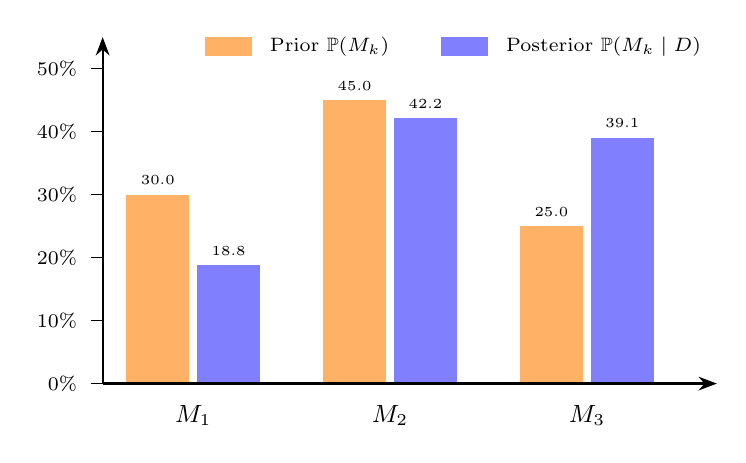
\begin{tikzpicture}[yscale=0.08]
    % --- Prior bars (left of each pair) ---
    \fill[orange!60] (0,0) rectangle (0.8, 30);
    \fill[orange!60] (2.5,0) rectangle (3.3, 45);
    \fill[orange!60] (5,0) rectangle (5.8, 25);

    % --- Posterior bars (right of each pair) ---
    \fill[blue!50] (0.9,0) rectangle (1.7, 18.75);
    \fill[blue!50] (3.4,0) rectangle (4.2, 42.19);
    \fill[blue!50] (5.9,0) rectangle (6.7, 39.06);

    % --- Axes ---
    \draw[thick, -{Stealth}] (-0.3,0) -- (7.5,0);
    \draw[thick, -{Stealth}] (-0.3,0) -- (-0.3,55);

    % Y-axis ticks
    \foreach \y in {0,10,20,30,40,50} {
      \draw (-0.45,\y) -- (-0.3,\y);
      \node[left, font=\scriptsize] at (-0.5,\y) {\y\%};
    }

    % X-axis labels
    \node[below, font=\small] at (0.85, -2) {$M_1$};
    \node[below, font=\small] at (3.35, -2) {$M_2$};
    \node[below, font=\small] at (5.85, -2) {$M_3$};

    % Value labels on bars
    \node[above, font=\tiny] at (0.4, 30)    {30.0};
    \node[above, font=\tiny] at (1.3, 18.75) {18.8};
    \node[above, font=\tiny] at (2.9, 45)    {45.0};
    \node[above, font=\tiny] at (3.8, 42.19) {42.2};
    \node[above, font=\tiny] at (5.4, 25)    {25.0};
    \node[above, font=\tiny] at (6.3, 39.06) {39.1};

    % Legend
    \fill[orange!60] (1, 52) rectangle (1.6, 55);
    \node[right, font=\scriptsize] at (1.7, 53.5) {Prior $\Prob(M_k)$};
    \fill[blue!50] (4, 52) rectangle (4.6, 55);
    \node[right, font=\scriptsize] at (4.7, 53.5) {Posterior $\Prob(M_k \given D)$};
  \end{tikzpicture}
  \caption{Prior vs.\ posterior probability for each machine.
           $M_3$'s posterior jumps from $25\%$ to $39\%$ due to its
           high defect rate.}
  \label{fig:bar}
\end{figure}

\end{sub}

% ----------------------------------------------------------
\subsection{Updating Beliefs Sequentially}
\label{sec:sequential}
% ----------------------------------------------------------
\begin{sub}

\begin{example}[Coin of unknown bias]
  \label{ex:coin}
  You are given a coin that is either fair ($\Prob(H) = 0.5$) or biased
  ($\Prob(H) = 0.8$), each equally likely \emph{a priori}.
  You flip it twice and observe $HH$.
  What is the posterior probability that the coin is biased?
\end{example}

\textbf{Solution.}
Let $B$ = ``coin is biased'' and $F$ = ``coin is fair.''
\begin{align*}
  \Prob(B) &= \Prob(F) = 0.5.
\end{align*}

The likelihood of $HH$ under each hypothesis (assuming independent flips):
\begin{align*}
  \Prob(HH \given B) &= 0.8^2 = 0.64, \\
  \Prob(HH \given F) &= 0.5^2 = 0.25.
\end{align*}

Applying Bayes' theorem:
\begin{align*}
  \Prob(B \given HH)
    &= \frac{\Prob(HH \given B)\,\Prob(B)}
            {\Prob(HH \given B)\,\Prob(B) + \Prob(HH \given F)\,\Prob(F)} \\[6pt]
    &= \frac{(0.64)(0.5)}{(0.64)(0.5) + (0.25)(0.5)} \\[6pt]
    &= \frac{0.32}{0.32 + 0.125} \\[6pt]
    &= \frac{0.32}{0.445}
     \approx \boxed{0.719}.
\end{align*}

After observing two heads, our belief shifts from $50\%$ to about $72\%$
in favor of the biased coin. Each subsequent observation would further
update the posterior --- this is the essence of \emph{Bayesian learning}.

If we continue flipping and keep getting heads, the posterior
$\Prob(B)$ evolves as shown below:

\begin{figure}[h]
  \centering
  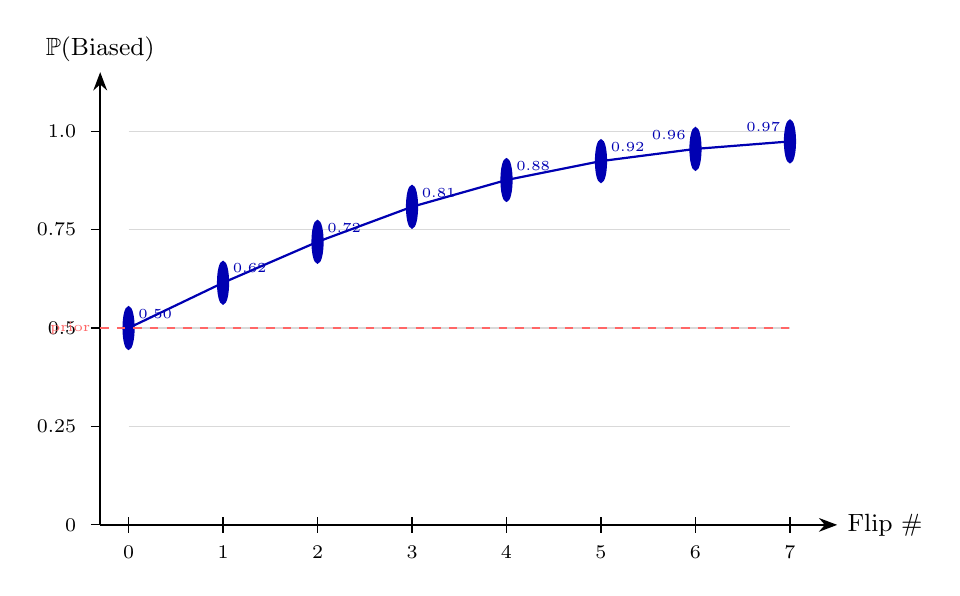
\begin{tikzpicture}[xscale=1.2, yscale=5]
    % Axes
    \draw[thick, -{Stealth}] (-0.3,0) -- (7.5,0)
      node[right, font=\small] {Flip \#};
    \draw[thick, -{Stealth}] (-0.3,0) -- (-0.3,1.15)
      node[above, font=\small] {$\Prob(\text{Biased})$};

    % Y ticks
    \foreach \y/\lab in {0/0, 0.25/0.25, 0.5/0.5, 0.75/0.75, 1.0/1.0} {
      \draw (-0.4,\y) -- (-0.3,\y);
      \node[left, font=\scriptsize] at (-0.45,\y) {\lab};
    }
    % Grid lines
    \foreach \y in {0.25, 0.5, 0.75, 1.0} {
      \draw[gray!30, thin] (0,\y) -- (7,\y);
    }

    % X ticks
    \foreach \x in {0,1,...,7} {
      \draw (\x,-0.02) -- (\x,0.02);
      \node[below, font=\scriptsize] at (\x,-0.03) {\x};
    }

    % Data: P(B) after 0..7 consecutive heads
    % 0: 0.500, 1: 0.615, 2: 0.719, 3: 0.808,
    % 4: 0.876, 5: 0.924, 6: 0.955, 7: 0.974
    \draw[thick, blue!70!black, mark=*, mark size=1.5pt]
      plot coordinates {
        (0, 0.500) (1, 0.615) (2, 0.719) (3, 0.808)
        (4, 0.876) (5, 0.924) (6, 0.955) (7, 0.974)
      };

    % Dot labels
    \node[above right, font=\tiny, blue!70!black] at (0, 0.500) {0.50};
    \node[above right, font=\tiny, blue!70!black] at (1, 0.615) {0.62};
    \node[above right, font=\tiny, blue!70!black] at (2, 0.719) {0.72};
    \node[above right, font=\tiny, blue!70!black] at (3, 0.808) {0.81};
    \node[above right, font=\tiny, blue!70!black] at (4, 0.876) {0.88};
    \node[above right, font=\tiny, blue!70!black] at (5, 0.924) {0.92};
    \node[above left,  font=\tiny, blue!70!black] at (6, 0.955) {0.96};
    \node[above left,  font=\tiny, blue!70!black] at (7, 0.974) {0.97};

    % Reference line
    \draw[dashed, red!60] (-0.3, 0.5) -- (7, 0.5);
    \node[left, font=\tiny, red!60] at (-0.3, 0.5) {prior};
  \end{tikzpicture}
  \caption{Sequential Bayesian updating: $\Prob(\text{Biased})$
           after observing $0, 1, 2, \ldots, 7$ consecutive heads.
           Each head shifts belief further toward the biased coin.}
  \label{fig:sequential}
\end{figure}

\end{sub}

% ==========================================================
\newpage
\section{Summary}
\label{sec:summary}
% ==========================================================

\begin{secbody}
\begin{itemize}
  \item Bayes' theorem \eqref{eq:bayes} converts
        $\Prob(\text{data} \given \text{hypothesis})$ into
        $\Prob(\text{hypothesis} \given \text{data})$.
  \item The proof relies only on the definition of conditional probability
        and the law of total probability.
  \item The prior matters: ignoring base rates leads to the
        \textbf{base rate fallacy} (Example~\ref{ex:medical}).
  \item Posteriors can be updated sequentially as new evidence arrives
        (Example~\ref{ex:coin}).
\end{itemize}
\end{secbody}

% ==========================================================
\newpage
\section{Homework Problems}
\label{sec:homework}
% ==========================================================

\begin{secbody}

% ---- Problem 4 ----
\textbf{Exercise 1.6.4.} \;
Find the reliability of the system below if each component has
reliability $0.92$.

\begin{center}
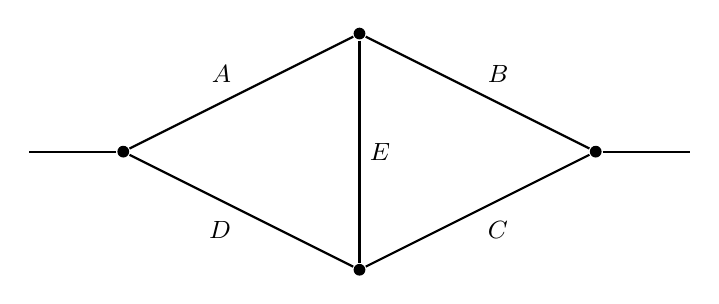
\begin{tikzpicture}[
  thick,
  dot/.style={fill, circle, inner sep=1.5pt},
]
  % Junction nodes
  \node[dot] (L)   at (0, 0)   {};
  \node[dot] (T)   at (3, 1.5) {};
  \node[dot] (B)   at (3,-1.5) {};
  \node[dot] (R)   at (6, 0)   {};

  % Input / output lines
  \draw (L) -- +(-1.2, 0);
  \draw (R) -- +( 1.2, 0);

  % Component A: L -> T (upper left)
  \draw (L) -- node[above left, font=\small] {$A$} (T);
  % Component B: T -> R (upper right)
  \draw (T) -- node[above right, font=\small] {$B$} (R);
  % Component D: L -> B (lower left)
  \draw (L) -- node[below left, font=\small] {$D$} (B);
  % Component C: B -> R (lower right)
  \draw (B) -- node[below right, font=\small] {$C$} (R);
  % Component E: T -> B (bridge)
  \draw (T) -- node[right, font=\small] {$E$} (B);
\end{tikzpicture}
\end{center}

% ---- Problem 8 ----
\bigskip
\textbf{Exercise 1.5.8.} \;
The following model is sometimes used to model the spread of a
contagious disease. Suppose a box contains $b$ black and $r$ red
marbles. A marble is drawn and $c$ marbles of that color together with
the drawn marble are replaced in the box before the next marble is
drawn, so that infected persons infect others while immunity to the
disease may also increase.
\begin{enumerate}
  \item[(a)] Find the probability that the first three marbles drawn
             are red.
  \item[(b)] Show that the probability of drawing a black on the second
             draw is the same as the probability of drawing a black on
             the first draw.
  \item[(c)] Show by induction that the probability the $k$th marble is
             black is the same as the probability of drawing a black on
             the first draw.
\end{enumerate}

% ---- Problem 16 ----
\bigskip
\textbf{Exercise 1.4.16.}
\begin{enumerate}
  \item[(a)] There is a fifty-fifty chance that firm A will bid for the
             construction of a bridge. Firm B submits a bid and the
             probability that it will get the job is $2/3$, provided
             firm A does not bid; if firm A submits a bid, the
             probability firm B gets the job is $1/5$. Firm B is
             awarded the job; what is the probability firm A did not
             bid?
  \item[(b)] In part (a), suppose now that the probability firm B gets
             the job if firm A bids on the job is $p$. Graph the
             probability that firm A did not bid given that B gets the
             job as a function of $p$.
  \item[(c)] Generalize parts (a) and (b) and further suppose that the
             probability that B gets the job given that firm A bids on
             the job is $r$. Graph the surface showing the probability
             firm A did not bid, given that firm B gets the job as a
             function of $p$ and $r$.
\end{enumerate}

% ---- Problem 21 ----
\bigskip
\textbf{Exercise 1.4.21.} \;
Three distinct methods, A, B, and C, are available for teaching a
certain industrial skill. The failure rates are $30\%$, $20\%$, and
$10\%$, respectively. However, due to costs, A is used twice as
frequently as B, which is used twice as frequently as C.
\begin{enumerate}
  \item[(a)] What is the overall failure rate in teaching the skill?
  \item[(b)] A worker is taught the skill, but fails to learn it
             correctly. What is the probability he was taught by
             method A?
\end{enumerate}

% ---- Problem 32 ----
\bigskip
\textbf{Exercise 1.4.32.} \;
A lie detector is accurate $3/4$ of the time. That is, if a person is
telling the truth, the lie detector indicates he is telling the truth
with probability $3/4$ while if the person is lying, the lie detector
indicates that he is lying with probability $3/4$. Assume that a person
taking the lie detector test is unable to influence its results and also
assume that $95\%$ of the people taking the test tell the truth. What is
the probability that a person is lying if the lie detector indicates
that he is lying?

\end{secbody}

\end{document}
